\documentclass[11pt]{article}
\usepackage[margin=1in]{geometry}
\usepackage{mathpazo}
\usepackage{amsmath,amssymb}
\usepackage{microtype}
\usepackage{booktabs}
\usepackage{graphicx}
\usepackage[dvipsnames]{xcolor}
\usepackage{tikz}
\usetikzlibrary{positioning,arrows.meta,calc,fit,backgrounds,decorations.pathreplacing}
\usepackage[most]{tcolorbox}
\usepackage{enumitem}
\usepackage[font=small,labelfont=bf]{caption}
\usepackage{hyperref}
\hypersetup{colorlinks=true,linkcolor=MidnightBlue,citecolor=MidnightBlue,urlcolor=MidnightBlue}
\usepackage{cleveref}
\urlstyle{tt}
\def\UrlBreaks{\do\_\do/\do.}
\newcommand{\file}[1]{\nolinkurl{#1}}
\newcommand{\code}[1]{\texttt{#1}}
\newcommand{\mhh}{m_{hh}}
\newcommand{\kl}{\kappa_\lambda}
\newcommand{\neff}{N_\text{eff}}
\newcommand{\stot}{\sigma_\text{tot}}

\definecolor{trainable}{HTML}{1B6CA8}
\definecolor{physics}{HTML}{2E933C}
\definecolor{datac}{HTML}{7B4EA3}
\definecolor{warn}{HTML}{C0392B}

\newtcolorbox{keyidea}[1][]{enhanced,breakable,colback=physics!6,colframe=physics!70!black,
  fonttitle=\bfseries,title={#1},boxrule=0.6pt,arc=2pt,left=6pt,right=6pt}
\newtcolorbox{aside}[1][]{enhanced,breakable,colback=trainable!5,colframe=trainable!70!black,
  fonttitle=\bfseries,title={#1},boxrule=0.6pt,arc=2pt,left=6pt,right=6pt}
\newtcolorbox{assume}[1][]{enhanced,breakable,colback=datac!5,colframe=datac!70!black,
  fonttitle=\bfseries,title={#1},boxrule=0.6pt,arc=2pt,left=6pt,right=6pt}
\newtcolorbox{watch}[1][]{enhanced,breakable,colback=warn!5,colframe=warn!70!black,
  fonttitle=\bfseries,title={#1},boxrule=0.6pt,arc=2pt,left=6pt,right=6pt}
\setlist{itemsep=2pt,topsep=3pt}

\title{\textbf{The \texttt{dihiggs} pipeline}\\[4pt]
\large Reproducibility, checks, the POWHEG noise, and training options}
\date{Working notes, October 26--29, 2026}

\begin{document}
\maketitle

\begin{abstract}
\noindent
These notes record a series of changes to, and studies of, the \code{dihiggs}
pipeline, which models the HEFT di-Higgs cross section in bins of $\mhh$ with a
physics-structured neural network (described in \file{docs/dihiggs_model.pdf}).
The pipeline was made runnable on Google Colab and reproducible, and the trained
model can now be exported as self-contained numpy and C++ code. A notebook of
checks confirms that the holdout spectra are disjoint from the training data and
that the test notebook compares like with like. The statistical noise in the POWHEG
spectra was then measured from the spectra themselves: every spectrum turns out to
be a histogram of \textbf{40,000} equal-weight events, not the 200,000 we were told.
Against that noise, the model agrees with POWHEG almost everywhere, with a median
$\chi^2$ per bin of 1.18, but misses real structure just above threshold. Finally,
the training notebook gained a choice of loss, an optional positivity constraint,
and a curriculum-learning variant, and their first tests are reported.
\end{abstract}

\begin{keyidea}[The main findings, for discussion]
\begin{enumerate}
  \item \textbf{The pipeline is reproducible and leak-free.} With the random seed
  fixed, \code{heft\_prepare\_data} gives the same split on every machine (holdout
  fingerprint \code{b610c204d33b}). The trained model records which training file it
  was trained on. All 25 checks pass.
  \item \textbf{Each POWHEG spectrum contains 40,000 events, not 200,000.} Every
  bin of every spectrum is a whole number of equal-weight events, so the events can
  be counted. The bin-to-bin fluctuations agree with that count. Ten spectra hold
  far fewer events and look like incomplete runs.
  \item \textbf{The model is about as accurate as POWHEG's own noise allows, except
  near threshold.} Typical differences are about 5\% per bin, which is the size of
  the noise itself. Above 555 GeV, the $\chi^2$ per bin is about 1.2. Between 255 and
  555 GeV it is 4, because the model misses the small plateau just above threshold
  and sometimes goes negative there.
  \item \textbf{Accuracy does not depend on the distance to the nearest training
  point,} over the range covered by the holdout set.
  \item \textbf{Training options.} A $\chi^2$ loss weighted by the POWHEG noise
  trained poorly. A positivity penalty reduces negative predictions. A curriculum
  starting with the small cross sections, especially with logarithmic pacing, does
  better on average in short runs, but by less than the spread between repeated runs.
\end{enumerate}
\end{keyidea}

\tableofcontents

% ===========================================================================
\section{What was done}
\label{sec:done}

\begin{center}
\small
\begin{tabular}{p{0.36\textwidth}p{0.58\textwidth}}
\toprule
item & where\\
\midrule
Notebooks run on Google Colab & a setup cell in every notebook; \code{USE\_DRIVE} shares \file{runs/} between notebooks\\
Self-contained copies of the model & \file{dihiggs/convert.py}, \file{code/heft_export.ipynb}: numpy and C++ versions\\
Description of the model & \file{docs/dihiggs_model.pdf}\\
Reproducible data split & \code{SEED} in \file{heft_prepare_data.ipynb}; fingerprints of the split and of the training file\\
Checks of the data and the test & \file{code/heft_checks.ipynb} (25 tests; plan in \file{docs/checks_plan.pdf})\\
Accuracy versus distance, and $\chi^2$ & new sections at the end of \file{heft_test.ipynb}\\
Choice of loss, positivity & switches in \file{heft_train.ipynb}\\
Curriculum learning & \file{code/heft_train_curriculum.ipynb}\\
Noise in the POWHEG spectra & this report (\cref{sec:noise})\\
\bottomrule
\end{tabular}
\end{center}

% ===========================================================================
\section{The pipeline and its provenance}
\label{sec:pipeline}

\Cref{fig:pipeline} shows how the data flow through the notebooks, and what each
step records so that later steps can verify where their inputs came from.

\begin{figure}[h]
\centering
\resizebox{\textwidth}{!}{%
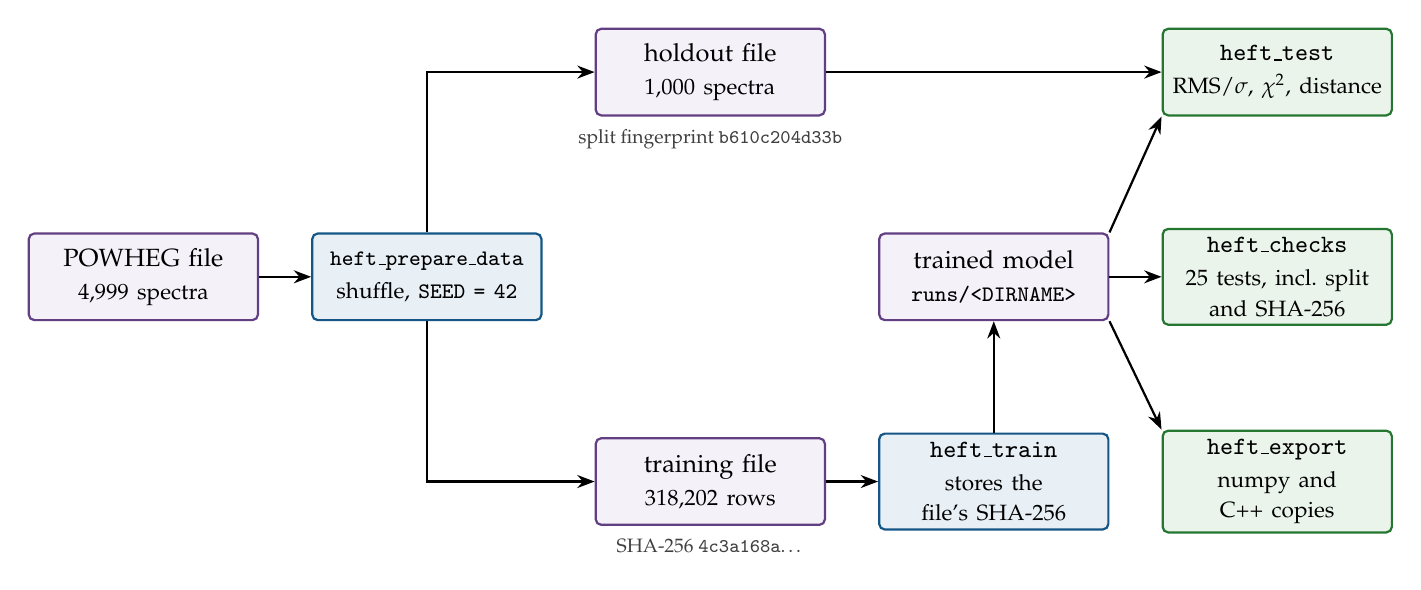
\begin{tikzpicture}[
  font=\small, >={Stealth[length=2.2mm]},
  box/.style={draw, rounded corners=2pt, thick, align=center, inner sep=3pt,
              minimum height=11mm, text width=27mm},
  dat/.style={box, fill=datac!8, draw=datac!80!black},
  nbk/.style={box, fill=trainable!10, draw=trainable!80!black},
  chk/.style={box, fill=physics!10, draw=physics!80!black},
  tag/.style={font=\scriptsize, text=black!75, align=center},
]
% columns at x = 0, 3.6, 7.2, 10.8, 14.4; rows at y = 2.6, 0, -2.6
\node[dat] (pw)     at (0, 0)      {POWHEG file\\[1pt]\footnotesize 4,999 spectra};
\node[nbk] (prep)   at (3.6, 0)    {{\footnotesize\code{heft\_prepare\_data}}\\[1pt]\footnotesize shuffle, \code{SEED = 42}};
\node[dat] (hold)   at (7.2, 2.6)  {holdout file\\[1pt]\footnotesize 1,000 spectra};
\node[dat] (train)  at (7.2, -2.6) {training file\\[1pt]\footnotesize 318,202 rows};
\node[nbk] (tr)     at (10.8, -2.6){\code{heft\_train}\\[1pt]\footnotesize stores the file's SHA-256};
\node[dat] (model)  at (10.8, 0)   {trained model\\[1pt]\footnotesize \code{runs/<DIRNAME>}};
\node[chk] (test)   at (14.4, 2.6) {\code{heft\_test}\\[1pt]\footnotesize RMS$/\sigma$, $\chi^2$, distance};
\node[chk] (checks) at (14.4, 0)   {\code{heft\_checks}\\[1pt]\footnotesize 25 tests, incl.\ split and SHA-256};
\node[chk] (export) at (14.4, -2.6){\code{heft\_export}\\[1pt]\footnotesize numpy and C++ copies};

\node[tag, below=1pt of hold]  {split fingerprint \code{b610c204d33b}};
\node[tag, below=1pt of train] {SHA-256 \code{4c3a168a}\dots};

\draw[->, thick] (pw) -- (prep);
\draw[->, thick] (prep.north) |- (hold.west);
\draw[->, thick] (prep.south) |- (train.west);
\draw[->, thick] (train) -- (tr);
\draw[->, thick] (tr) -- (model);
\draw[->, thick] (hold) -- (test);
\draw[->, thick] (model.north east) -- (test.south west);
\draw[->, thick] (model) -- (checks);
\draw[->, thick] (model.south east) -- (export.north west);
\end{tikzpicture}}
\caption{The data flow (solid arrows) and what each step records. The split into
holdout and training spectra is fixed by \code{SEED}. Its fingerprint, a code
computed from the sorted IDs of the holdout spectra, shows at a glance whether two
runs made the same split. The training notebook stores the SHA-256 of the training
file in the model's configuration, so \code{heft\_checks} can confirm that a saved model
was trained on the data that are now on disk, and that the holdout and training files
come from the same split.}
\label{fig:pipeline}
\end{figure}

\subsection{Why the seed mattered}

\code{heft\_prepare\_data} shuffles the spectra before setting aside the first 1,000
for testing. Without a fixed seed, every run made a different split. The holdout and
training files are written together, so a single run is self-consistent. But if the
training file of one run were ever paired with the holdout file of another, which
the separate git commits ``update traindata'' and ``update testdata'' made possible,
each holdout spectrum would be in the other run's training set with probability 3,999/4,999, so about four fifths of the holdout spectra would also be training spectra. The test would
then measure memory, not generalisation.

The fix has three parts:
\begin{itemize}
  \item \textbf{A fixed seed} for both shuffles. Each shuffle builds its own generator
  from the seed, so rerunning a single cell gives the same result. The generator is
  numpy's \code{RandomState}, whose sequence of random numbers is frozen across numpy
  versions, so the split is the same on every machine. Two different machines
  gave the same fingerprint, \code{b610c204d33b}.
  \item \textbf{Byte-identical files.} The training file is gzipped without a time
  stamp, so rerunning the notebook does not create spurious changes in git.
  \item \textbf{A link from model to data.} \code{heft\_train} saves the SHA-256 of
  the training file in the model's configuration.
\end{itemize}

\subsection{The checks}

\code{heft\_checks.ipynb} reads the files, changes nothing, and prints PASS or FAIL
for each of 25 tests. On the current data and model, \textbf{all 25 pass}:

\begin{center}
\small
\begin{tabular}{lp{0.7\textwidth}}
\toprule
group & what is confirmed\\
\midrule
1. unique points & no two POWHEG rows share their Wilson coefficients, exactly or to within $10^{-6}$ (in units of each coefficient's spread); no two share a spectrum\\
2. disjoint sets & the holdout and training files share no ID and no parameter point; together they contain every POWHEG spectrum once; every value in both files equals the POWHEG file; the training notebook reads only the training file; the model was trained on the current training file\\
3. the test & \code{heft\_test} compares each POWHEG spectrum with the model's prediction for the same point, at the right masses, after sorting; this is confirmed against an independent calculation with the exported numpy model\\
\bottomrule
\end{tabular}
\end{center}

The nearest two parameter points are 0.11 apart in those units, and the typical
spacing is about 0.45. So there are no near-duplicates.

% ===========================================================================
\section{Self-contained copies of the model}
\label{sec:export}

\code{dihiggs.convert} writes the trained parameters to a plain-text file and copies
two hand-written, commented implementations next to it:
\begin{itemize}
  \item \file{heftnet_numpy.py}, which needs only numpy;
  \item \file{heftnet.hpp}, a header-only C++17 file that uses only the standard
  library and works in ROOT. Its comments explain the newer C++ constructs.
\end{itemize}
Both take $\mhh$ in GeV and return the cross section in pb per 15 GeV bin. The weights
are written with enough digits to be read back exactly, and the converter checks both
copies against the PyTorch model, which they reproduce to about $10^{-11}$.

\begin{assume}[Assumption: the mass variable]
The network's input is the dimensionless $x$, with bins of width 0.01. The POWHEG
histograms start at 0 GeV with 15 GeV bins (confirmed), and bins 17--96 are used, so
\[
  \mhh = 255~\text{GeV} + 1500~\text{GeV} \times x , \qquad 255 \le \mhh < 1455~\text{GeV}.
\]
Outside that range the copies extrapolate; the numpy copy warns.
\end{assume}

% ===========================================================================
\section{How accurate is the model?}
\label{sec:accuracy}

\subsection{What RMS$/\sigma$ measures}

For a spectrum with POWHEG cross sections $f_k$ and predictions $y_k$ in its 80 bins,
\[
  \frac{\text{RMS}}{\sigma} = \frac{1}{\sigma_\text{tot}} \sqrt{\frac{1}{80}\sum_{k=1}^{80} (y_k - f_k)^2}
  = \frac{\sqrt{\text{bias}^2 + \text{variance}}}{\sigma_\text{tot}} .
\]
The typical value is $6 \times 10^{-4}$, which sounds tiny. But the numerator is a
\emph{per-bin} difference and the denominator is the sum of 80 bins. Since a typical
bin holds about 1/80 of the total, $6\times10^{-4}$ of the total is about 5\% of a
typical bin. That is the size of POWHEG's bin-to-bin noise (\cref{sec:noise}), and it
is why the comparisons look so good by eye: the model runs through the middle of the
noise.

\subsection{Why the holdout set should be random}

It is tempting to choose holdout points as far as possible from the training points,
to make the test harder. In five dimensions with 20\% held out, this backfires:

\begin{center}
\small
\begin{tabular}{lp{0.21\textwidth}p{0.17\textwidth}p{0.17\textwidth}}
\toprule
holdout choice & distance to the nearest training point & distance from the centre & outermost training point\\
\midrule
random (as now) & median 0.50 (0.13--1.59) & median 2.08 & 4.62\\
1,000 most isolated & median 0.85 (0.65--2.41) & median 2.95 & 4.11\\
\bottomrule
\end{tabular}
\end{center}

(Distances are in units of each coefficient's standard deviation.) The most isolated
points are those in the outer parts of the Gaussian cloud. Holding them out shrinks
the training region, so the test measures \emph{extrapolation}. A random holdout
instead gives an unbiased estimate of the accuracy a colleague will see at points
drawn from the same region.

\subsection{Accuracy versus distance from the training points}

Because the holdout points are random, some lie close to a training point and others
far from all of them. \Cref{fig:distance} shows that neither RMS$/\sigma$ nor $\chi^2/N$
(\cref{sec:chi2}) depends on that distance. The rank correlations are $-0.00$ and
$+0.02$, and the closest and farthest quarters of the holdout points have the same
median RMS$/\sigma$ ($6.10$ and $6.09 \times 10^{-4}$).

\begin{figure}[h]
\centering
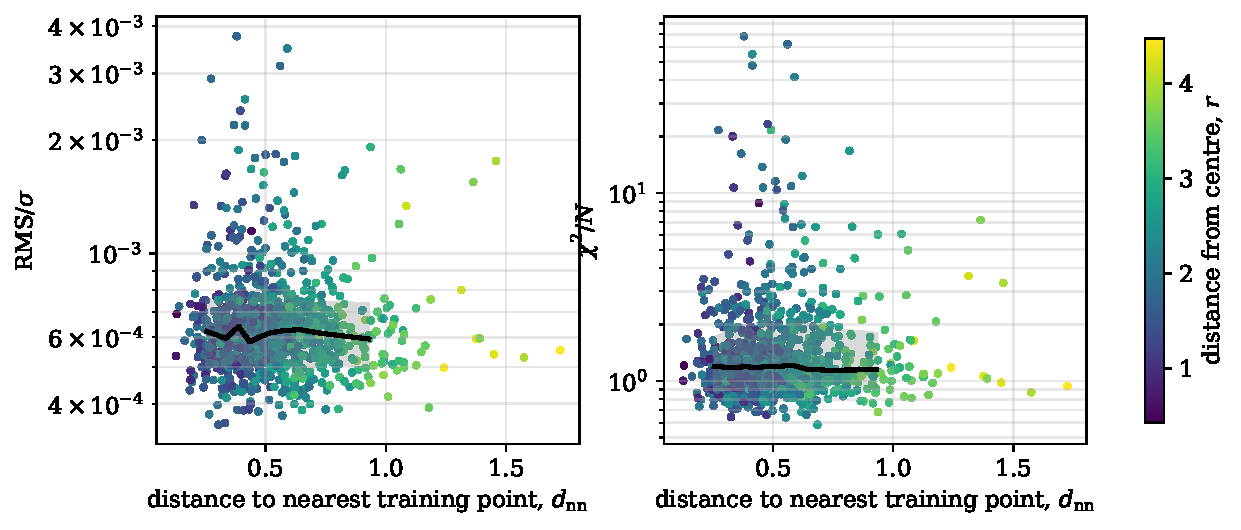
\includegraphics[width=0.92\textwidth]{fig_distance.pdf}
\caption{Accuracy of the fully trained model on the 1,000 holdout spectra against the
distance to the nearest of the 3,999 training points. Each dot is one spectrum,
coloured by its distance from the centre of the training points. The black line is
the median in ten bins of distance, and the grey band holds the middle 68\%.}
\label{fig:distance}
\end{figure}

\begin{aside}[Why a flat curve is not the end of the story]
When most of the differences between model and POWHEG are POWHEG's own noise
(\cref{sec:chi2}), RMS$/\sigma$ is dominated by the noise, and any dependence on
distance is hidden beneath it. The $\chi^2$, which divides out the noise, is also
flat. So within the range of distances covered, 0.13 to 1.7, the model interpolates
equally well everywhere.
\end{aside}

% ===========================================================================
\section{The noise in the POWHEG spectra}
\label{sec:noise}

POWHEG gives no uncertainty for each bin. To judge the model we need one, so we
measured it from the spectra themselves. The result was then checked against what the
colleague who generated the spectra told us: 200,000 events per spectrum.

\subsection{Step 1: the bin-to-bin jitter}

For a smooth spectrum, a bin and the average of its two neighbours are nearly equal,
so their difference is mostly noise (\cref{fig:jitter}).

\begin{figure}[h]
\centering
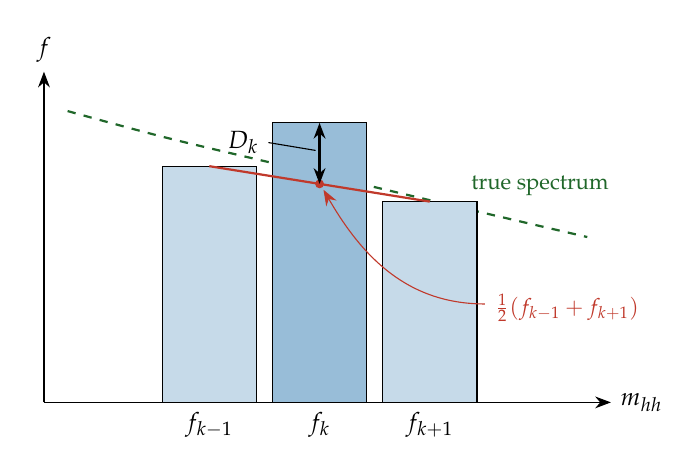
\begin{tikzpicture}[scale=1.0, >={Stealth[length=2mm]}, font=\small]
  \draw[->] (0,0) -- (7.2,0) node[right] {$\mhh$};
  \draw[->] (0,0) -- (0,4.2) node[above] {$f$};
  % smooth truth
  \draw[thick, physics!70!black, dashed] plot[smooth] coordinates {(0.3,3.7) (1.6,3.35) (3.5,2.9) (5.4,2.45) (6.9,2.1)};
  \node[physics!70!black, font=\footnotesize] at (6.3,2.75) {true spectrum};
  % bars
  \fill[trainable!25] (1.5,0) rectangle (2.7,3.0);
  \fill[trainable!45] (2.9,0) rectangle (4.1,3.55);
  \fill[trainable!25] (4.3,0) rectangle (5.5,2.55);
  \draw (1.5,0) rectangle (2.7,3.0);  \draw (2.9,0) rectangle (4.1,3.55);  \draw (4.3,0) rectangle (5.5,2.55);
  \node[below] at (2.1,0) {$f_{k-1}$}; \node[below] at (3.5,0) {$f_k$}; \node[below] at (4.9,0) {$f_{k+1}$};
  % average of neighbours
  \draw[thick, warn] (2.1,3.0) -- (4.9,2.55);
  \fill[warn] (3.5,2.775) circle (1.6pt);
  \node[warn, font=\footnotesize, anchor=west] at (5.6,1.2) {$\tfrac12(f_{k-1} + f_{k+1})$};
  \draw[warn, ->, thin] (5.6,1.25) to[out=180, in=-60] (3.55,2.7);
  % D_k
  \draw[<->, thick] (3.5,2.775) -- (3.5,3.55);
  \node[anchor=east] at (2.85,3.3) {$D_k$};
  \draw[thin] (2.85,3.3) -- (3.45,3.2);
\end{tikzpicture}
\caption{The jitter $D_k = f_k - \tfrac12(f_{k-1} + f_{k+1})$. For a smooth spectrum,
the average of the neighbours (red) is close to the true value at bin $k$, so $D_k$ is
mostly noise. Where the spectrum curves sharply, near threshold and near the peak,
$D_k$ also contains a contribution from the curvature.}
\label{fig:jitter}
\end{figure}

\subsection{Step 2: the jitter behaves like counting noise}

If a spectrum is a histogram of $N$ events, bin $k$ holds on average
$n_k = N f_k / \stot$ of them, where $\stot = \sum_k f_k$. Counting statistics then give
a relative error of $1/\sqrt{n_k}$, that is
\[
  \sigma_k^2 = \frac{f_k\,\stot}{N} .
\]
The relative noise should therefore fall as the inverse square root of the fraction of
the spectrum in the bin. The left panel of \cref{fig:noise} shows that it does, over
more than two decades. The data lie on the line for 40,000 events, not on the one for
200,000.

Measuring $N$ precisely uses the jitter itself. With independent noise, the variance
of $D_k$ is $\sigma_k^2 + \tfrac14\sigma_{k-1}^2 + \tfrac14\sigma_{k+1}^2$, so
\[
  q_k = \frac{D_k^2}{\stot\,\big(f_k + \tfrac14(f_{k-1} + f_{k+1})\big)}
\]
is $1/N$ times the square of a standard Gaussian variable, whose median is 0.455.
Hence $N = 0.455 / \text{median}(q_k)$. The median, rather than the mean, is not pulled
by the few bins with large curvature. Using all 4,999 spectra and the bins above
570 GeV, where they are smooth, gives $\neff \approx 38{,}000$.

\textbf{A closure test} confirms that the method works. Spectra simulated with exactly
200,000 equal-weight events give an estimate of 171,000. Spectra with 38,000 events
give 36,000. So the method reads slightly low, and the real spectra correspond to
about 40,000 events, a fifth of 200,000.

\begin{figure}[t]
\centering
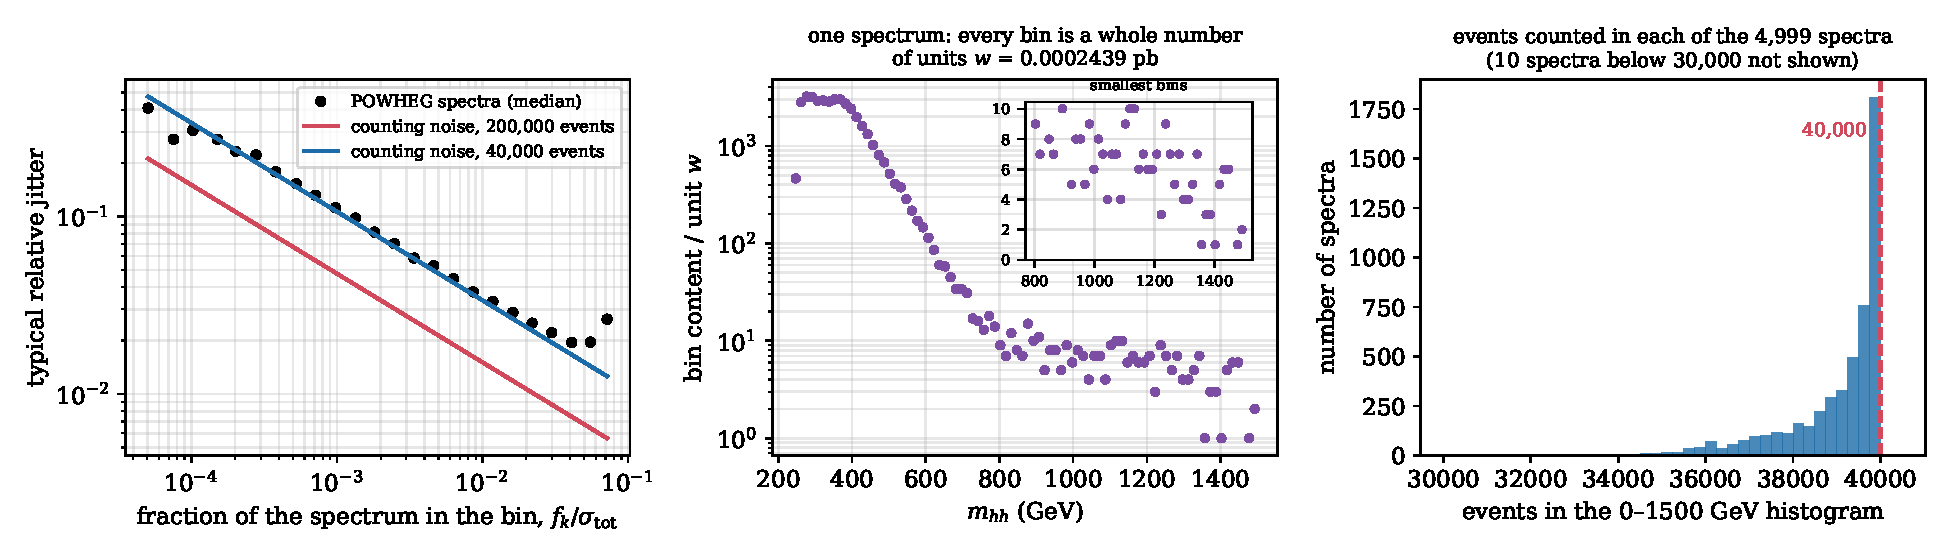
\includegraphics[width=\textwidth]{fig_noise.pdf}
\caption{Left: the typical relative jitter of the POWHEG bins against the fraction of
the spectrum in the bin, with the expectation for counting noise from 200,000 (red)
and 40,000 (blue) events. Middle: one spectrum, with every bin divided by that
spectrum's smallest unit $w$. Every bin is a whole number, and the inset shows the
smallest. Right: the number of events counted in each spectrum. None has more than
40,000, and the shortfall is the events above 1500 GeV.}
\label{fig:noise}
\end{figure}

\subsection{Step 3: counting the events}

A histogram of equal-weight events has a striking property: every bin is a whole
number of events times the weight of one event, $w$. So the bin contents should be
\emph{integer multiples of a common unit}. They are, in all 4,999 spectra. The
largest departure of any bin from a whole number of units is 0.0009 (middle panel of
\cref{fig:noise}). Dividing each spectrum's total by its unit counts its events:

\begin{itemize}
  \item \textbf{No spectrum has more than 40,000 events.} The median is 39,524, in the
  0--1500 GeV histogram.
  \item \textbf{The shortfall is overflow.} The number of missing events tracks the
  number in the top bin (rank correlation $+0.97$). So the missing events are those
  above 1500 GeV, which the histogram does not record.
  \item \textbf{The counts agree with the jitter.} The noise model of Step 2 gives
  variances within about 3\% of exact counting noise for a typical spectrum.
  \item \textbf{The spectra are independent.} The fluctuations of neighbouring
  parameter points are uncorrelated (correlation $+0.004$). So the spectra were not
  made by reweighting one common sample.
  \item \textbf{The noise is the same everywhere.} $\neff$ does not depend on $\theta$
  or on $\stot$. Its spread from spectrum to spectrum is exactly what estimation noise
  alone produces.
\end{itemize}

\begin{watch}[Ten anomalous spectra]
Ten spectra have far fewer than 40,000 events, even allowing for events above
1500 GeV. They look like incomplete runs, and their noise is much larger than that of
the others. Two are in the holdout set.
\begin{center}
\small
\begin{tabular}{lcccccccccc}
\toprule
ID & 2841 & 4959 & 984 & 4850 & 4317 & 4321 & 1965 & 3571 & 3207 & 805\\
events & 1,348 & 11,876 & 12,078 & 13,808 & 19,136 & 23,937 & 24,865 & 25,741 & 33,814 & 34,269\\
holdout & yes & & & & & & & & & yes\\
\bottomrule
\end{tabular}
\end{center}
\end{watch}

\begin{assume}[Assumptions in this section]
\begin{itemize}
  \item The bins' noise is independent from bin to bin. It is: after the same light
  smoothing, the residuals of adjacent bins correlate at $-0.29$ in the data and at
  $-0.28$ in spectra simulated with independent counting noise, a correlation that the
  smoothing itself produces.
  \item Each spectrum comes from one run of equal-weight events, with no negative
  weights. The exact integer quantization of every bin makes this certain.
  \item ``200,000 events'' must then refer to something else, such as events generated
  before a selection, or the total over five runs. \textbf{This needs to be clarified
  with the colleague who generated the spectra.}
\end{itemize}
\end{assume}

% ===========================================================================
\section{Is the model consistent with the noise?}
\label{sec:chi2}

\subsection{The $\chi^2$ per bin}

RMS$/\sigma$ says how large the differences are, but not whether they are larger than
the noise. That question is answered by
\[
  \frac{\chi^2}{N} = \frac{1}{N}\sum_{k=1}^{N} \left( \frac{y_k - f_k}{\sigma_k} \right)^2 ,
\]
over the $N$ bins with $f_k > 0$, with $\sigma_k$ from \cref{sec:noise}. Each term is a
squared difference in units of the noise. If the model were exact, $\chi^2/N$ would
scatter around 1 with a standard deviation of $\sqrt{2/N} \approx 0.16$.

\begin{aside}[Why the eye and the numbers seem to disagree]
\begin{itemize}
  \item \textbf{The noise is smallest where the eye is least sensitive.} With 40,000
  events, a bin at the peak holding 5\% of the spectrum has a relative noise of only
  about 2\%. A 5\% miss there is a $2\sigma$ deviation, but it is invisible on a linear
  plot scaled to the peak.
  \item \textbf{$\chi^2/N$ near 1 means the model is better than the noise.} If the
  model's own error per bin is $\delta$, then on average $\chi^2/N = 1 + (\delta/\sigma)^2$.
  The median, 1.18, means $\delta \approx \sqrt{0.18}\,\sigma \approx 0.4\,\sigma$: the
  model's error is less than half of POWHEG's statistical precision.
\end{itemize}
\end{aside}

\subsection{Results for the fully trained model}

\begin{center}
\small
\begin{tabular}{lcc}
\toprule
 & holdout spectra & if the model matched POWHEG within the noise\\
\midrule
median $\chi^2/N$ & 1.18 & 1\\
middle 68\% & 0.92--1.94 & 0.84--1.16\\
spectra with $\chi^2/N > 2$ / $> 5$ & 15\% / 3.5\% & almost none\\
mean $\chi^2$ per bin, 255--555 GeV & \textbf{4.0} & 1\\
mean $\chi^2$ per bin, 555--1005 GeV & 1.2 & 1\\
mean $\chi^2$ per bin, 1005--1455 GeV & 1.2 & 1\\
\bottomrule
\end{tabular}
\end{center}

\begin{figure}[h]
\centering
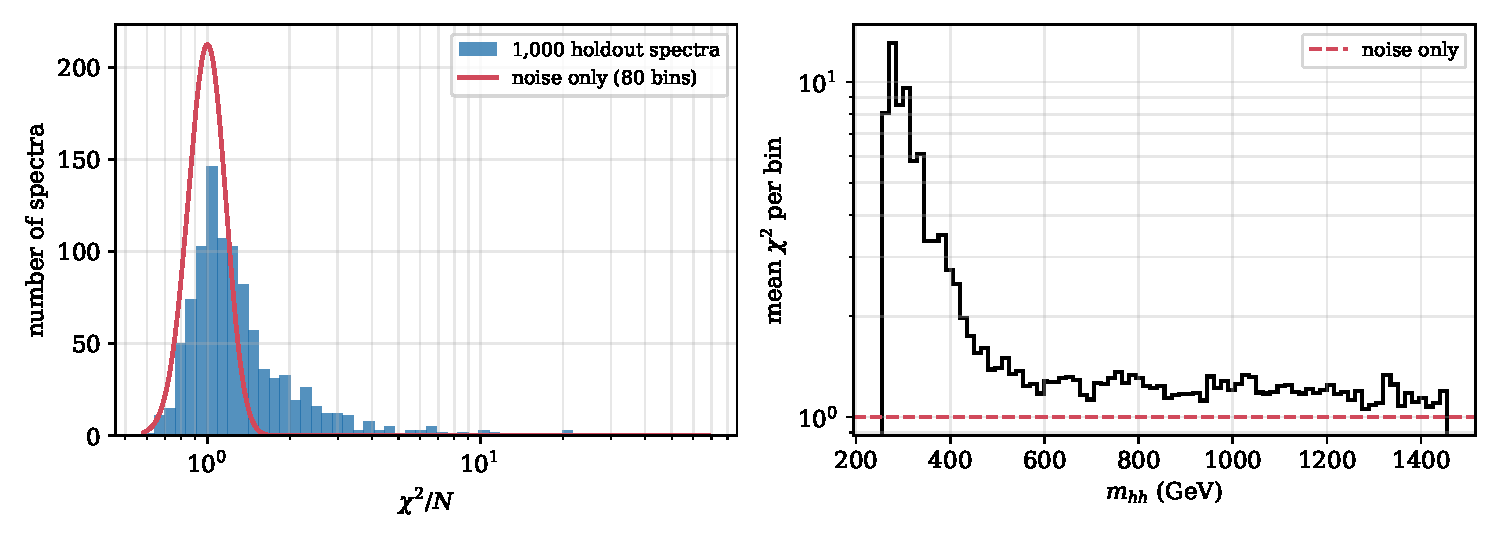
\includegraphics[width=0.95\textwidth]{fig_chi2.pdf}
\caption{Left: the distribution of $\chi^2/N$ over the holdout spectra, with the
expectation if the model matched POWHEG within the noise (red). Right: the mean
$\chi^2$ per bin against $\mhh$. Above about 450 GeV it is close to 1. Near threshold
it rises to about 10.}
\label{fig:chi2}
\end{figure}

\begin{figure}[h]
\centering
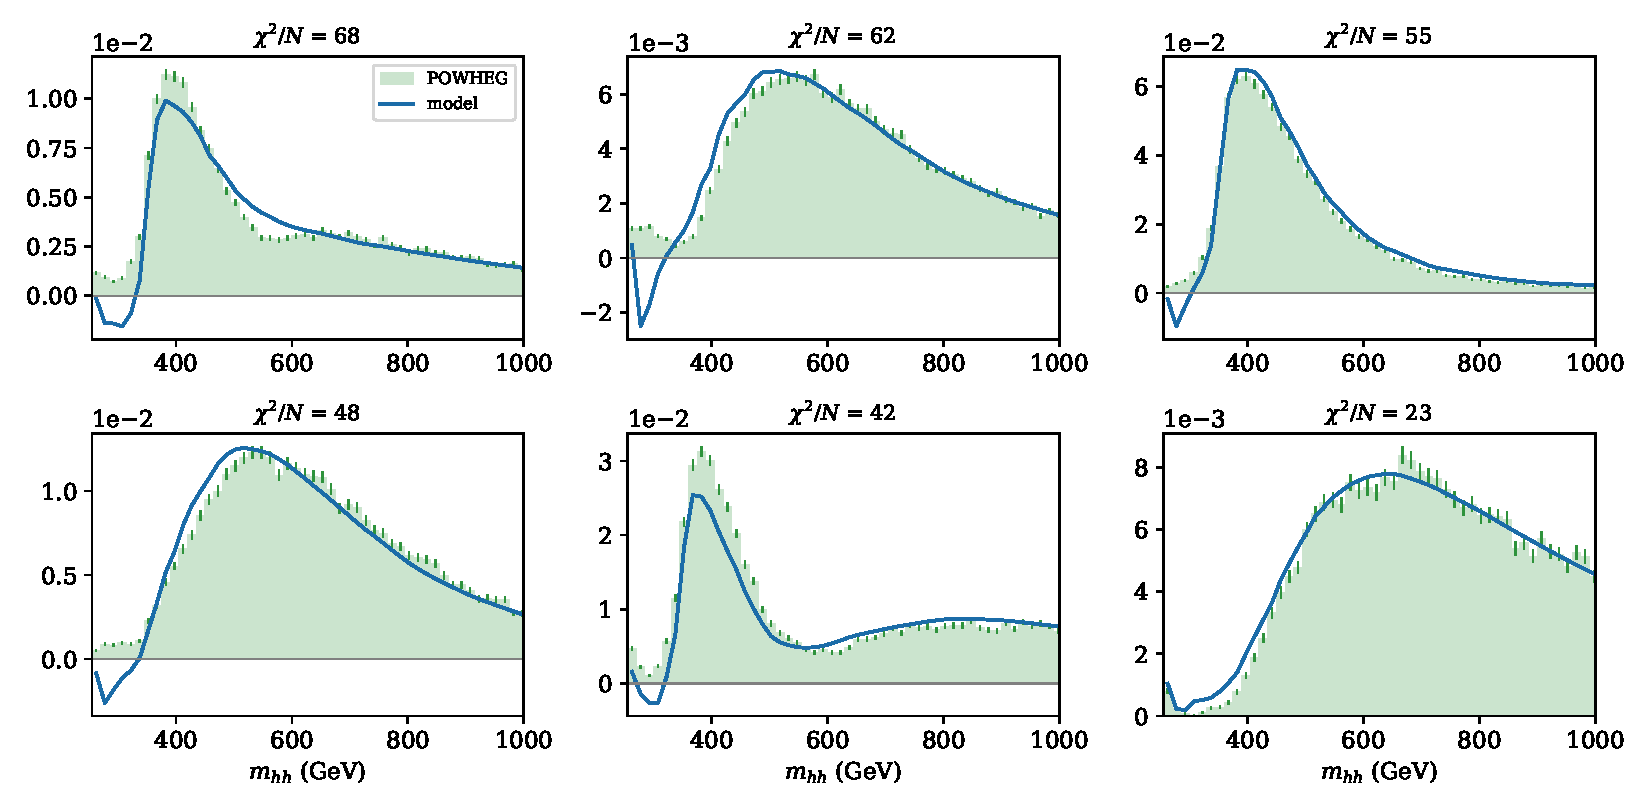
\includegraphics[width=0.95\textwidth]{fig_worst.pdf}
\caption{The six holdout spectra with the largest $\chi^2/N$, with the estimated noise
as error bars. In the first few bins above threshold, POWHEG has a small positive
plateau. The model dips below it, sometimes to a negative cross section, and in some
spectra it misses the height of a sharp peak.}
\label{fig:worst}
\end{figure}

The pulls, $(y_k - f_k)/\sigma_k$, have mean $+0.02$ and median absolute value 0.73,
against 0.67 for a standard Gaussian. So the noise model describes the bulk of the bins
well. Their standard deviation, 1.4, comes from the tail near threshold. $\chi^2/N$ is
worse for spectra with a smaller total cross section (rank correlation $-0.38$). The
fully trained model predicts a negative cross section in 100 of the 80,000 holdout bins,
the most negative being $-0.014$ pb.

% ===========================================================================
\section{Training options}
\label{sec:training}

\subsection{Three losses}

\code{heft\_train} now has a switch, \code{LOSS}:

\begin{center}
\small
\begin{tabular}{lll}
\toprule
\code{LOSS} & loss per row & weighting\\
\midrule
\code{'L1'} & $\lvert f - t \rvert / S$ & every pb counts the same; the minimum is the median\\
\code{'MSE'} & $(f - t)^2 / S^2$ & every pb counts the same; the minimum is the mean\\
\code{'CHI2'} & $(f - t)^2 / \sigma_k^2$ & each bin weighted by its POWHEG precision\\
\bottomrule
\end{tabular}
\end{center}

Here $S \approx 0.012$ pb is the median cross section of the training rows. Dividing
by it makes the losses dimensionless without changing the minimum. With L1 or MSE,
the training is dominated by the largest cross sections. CHI2 is the statistician's
choice, but in tests it trained poorly:

\begin{center}
\small
\begin{tabular}{lccc}
\toprule
20,000 iterations & holdout median $\chi^2/N$ & median RMS$/\sigma$ & negative bins\\
\midrule
L1 & 3.8 & $1.3 \times 10^{-3}$ & 3.3\%\\
CHI2 & 382 & $2.0 \times 10^{-2}$ & 1.1\%\\
CHI2, learning rate $\div 10$ & 454 & $2.1 \times 10^{-2}$ & --\\
\bottomrule
\end{tabular}
\end{center}

Two problems were found:
\begin{itemize}
  \item \textbf{Nearly empty bins.} The noise model gives a tiny $\sigma_k$ to bins
  expected to hold less than one event, and their huge weights made the training
  unstable. Adding the variance of one event,
  $\sigma_k^2 = (f_k + \stot/\neff)\,\stot/\neff$, cured the instability.
  \item \textbf{Poor conditioning remains.} The weights span about ten orders of
  magnitude, because $\sigma_k^2$ grows with $\stot^2$ and the totals range from
  $10^{-3}$ to 400 pb. The loss then demands the same relative precision across
  spectra whose sizes differ by five orders of magnitude. A smaller learning rate did
  not help. CHI2 is kept in the notebook, marked experimental.
\end{itemize}

\subsection{A positivity constraint}

A cross section is an integral of $|\mathcal{M}|^2$, so it cannot be negative for any
$\theta$. With \code{POSITIVITY = True}, the loss gains a penalty,
\[
  R = R_\text{data} + \lambda\,\frac{1}{M}\sum_{j=1}^{M}\left(\frac{\max(0, -f_j)}{S}\right)^2 ,
\]
evaluated at $M = 2048$ \emph{random} parameter points per iteration. Positivity must
hold everywhere, not only at the training points, and the negative predictions we
found were at unseen points. A hard constraint, such as passing the output through a
positive function, would destroy the exact polynomial dependence on $\theta$, which is
the heart of the model. The penalty keeps that structure exact. In short tests of
3,000 iterations, it cut the share of negative predictions at random points from 20\%
to 5\% with L1, from 17\% to 14\% with MSE, and from 45\% to 19\% with CHI2. Full runs
are needed to choose $\lambda$.

% ===========================================================================
\section{Curriculum learning}
\label{sec:curriculum}

\code{heft\_train\_curriculum.ipynb} is \code{heft\_train} with one change: the training
rows are presented in order of increasing cross section. The idea, due to Bengio
\emph{et al.} (2009), is that a network may learn better when it meets easy examples
first. Here the motivation is specific. With L1, the large cross sections dominate the
loss from the first iteration, and the small ones are where the model is weakest.
Starting with the small ones gives them the network's full attention first.

\begin{itemize}
  \item \textbf{Ordering} (\code{CURRICULUM\_BY}): by the cross section of the bin,
  or by the total of the spectrum.
  \item \textbf{Pacing:} at iteration $i$, batches are drawn from the rows below a
  threshold that rises until all rows are available, by default halfway through the
  run. Only the training rows are reordered; validation is unchanged.
\end{itemize}

\begin{figure}[h]
\centering
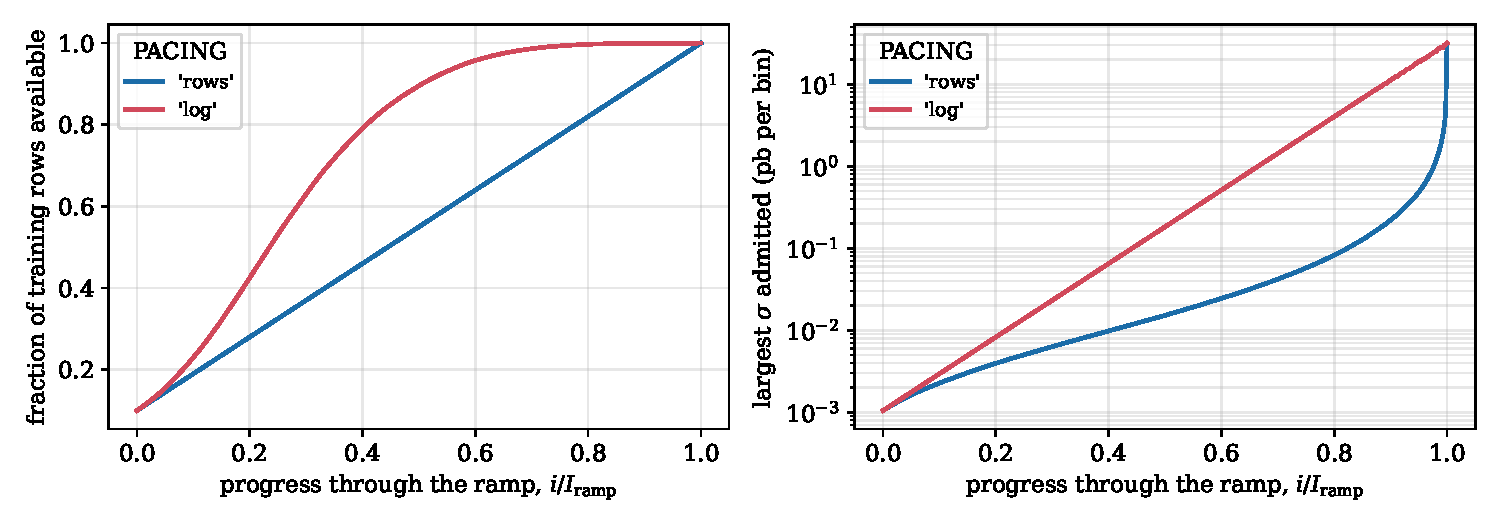
\includegraphics[width=0.92\textwidth]{fig_pacing.pdf}
\caption{The two pacings, for the per-bin ordering. With \code{'rows'}, the fraction of
rows grows linearly (left), but because most rows have small cross sections, the
largest cross sections arrive almost at once at the end (right). With \code{'log'}, the
largest admitted cross section grows by the same factor in each stage of the ramp, so
large cross sections are introduced as gradually as small ones.}
\label{fig:pacing}
\end{figure}

\paragraph{Results.} Runs of 20,000 iterations with the per-bin ordering, evaluated on
the holdout spectra. Training is not seeded, so repeated runs differ, and the table
shows the mean and the range over the repeats.

\begin{center}
\small
\begin{tabular}{lccccc}
\toprule
 & median & $\chi^2/N$, smallest & median & mean $\chi^2$ per bin, & negative\\
setting (3 runs each) & $\chi^2/N$ & 25\% of spectra & RMS$/\sigma$ ($10^{-3}$) & 255--555 GeV & bins\\
\midrule
plain L1 & 4.6 (3.8--6.1) & 19 (8--30) & 1.36 (1.12--1.66) & 108 (36--185) & 2.6\%\\
curriculum, \code{'rows'} & 4.0 (2.6--5.8) & 13 (9--20) & 1.21 (0.96--1.39) & 68 (45--81) & 1.6\%\\
curriculum, \code{'log'} & 3.1 (2.3--3.6) & 10 (6--13) & 1.12 (1.01--1.18) & 57 (24--79) & 1.9\%\\
\bottomrule
\end{tabular}
\end{center}

\begin{figure}[h]
\centering
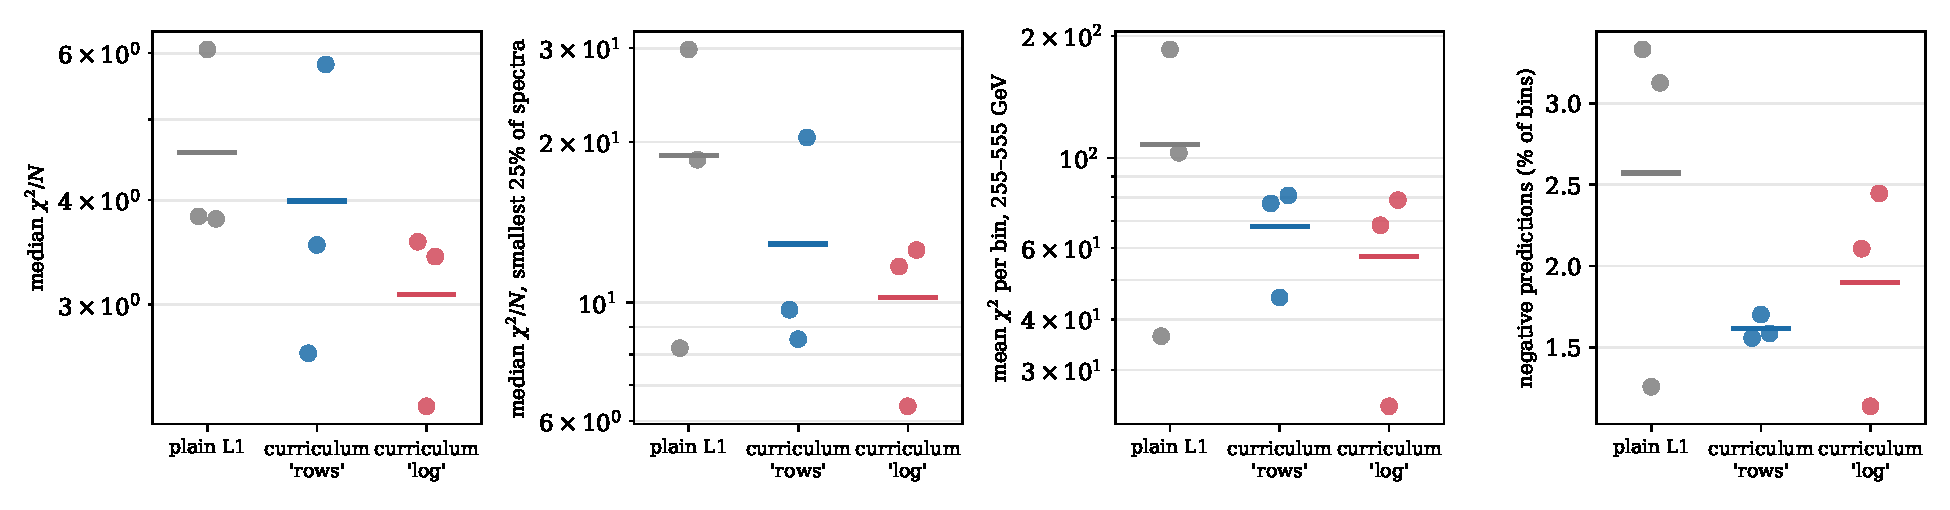
\includegraphics[width=\textwidth]{fig_curriculum.pdf}
\caption{Every run of the comparison, one dot per run; the lines mark the means. The
spread between identical runs is as large as the differences between settings.}
\label{fig:curriculum}
\end{figure}

\paragraph{What the comparison shows.}
\begin{itemize}
  \item \textbf{On average, both curricula do better than plain L1 on every measure}:
  overall, for the smallest spectra, near threshold, and in the number of negative
  predictions. Log pacing does a little better than row pacing.
  \item \textbf{The evidence is weak.} The spread between identical runs is as large as
  the differences between settings (\cref{fig:curriculum}), there are only three runs of
  each, and each run is a tenth of a full training run. For comparison, the fully trained
  model reaches a median $\chi^2/N$ of 1.18.
  \item \textbf{The decisive test} is full-length runs of plain L1 and of the curriculum
  with log pacing, preferably with the training seeded, so that differences between
  settings are not confused with differences between runs.
\end{itemize}

% ===========================================================================
\section{Open questions and next steps}
\label{sec:next}

\begin{enumerate}
  \item \textbf{For the colleague who made the spectra.}
  \begin{itemize}
    \item What does ``200,000 events'' refer to, when each histogram holds 40,000?
    \item Did the runs for the ten short spectra finish?
    \item Is there a reason the histograms stop at 1500 GeV? About 1\% of the events lie
    above, and up to 10\% in some spectra.
  \end{itemize}
  \item \textbf{Use the exact noise.} Each bin's event count is $n_k = f_k/w$, so the
  exact noise is $\sigma_k = w\sqrt{n_k}$. This could replace the estimate of $\neff$ in
  \code{heft\_test} and the CHI2 loss, and would automatically give the ten short spectra
  their larger noise.
  \item \textbf{The threshold region} is where the model falls short. Possible remedies:
  \begin{itemize}
    \item the positivity penalty, in full runs;
    \item a loss that weights the threshold bins more without the conditioning problem of
    CHI2, for example $\chi^2$ normalised per spectrum;
    \item including the threshold bin 16 (240--255 GeV), which is now dropped.
  \end{itemize}
  \item \textbf{Seed the training} (weight initialisation and batch sampling), so that
  runs can be compared without repeats.
  \item \textbf{Full-length runs} (200,000 iterations) of the most promising options,
  compared with \code{heft\_test}.
\end{enumerate}

% ===========================================================================
\appendix
\section{The notebooks, and the order in which to run them}

\begin{center}
\small
\begin{tabular}{lp{0.36\textwidth}p{0.48\textwidth}}
\toprule
step & notebook & what it does\\
\midrule
1 & \file{heft_prepare_data.ipynb} & writes the holdout and training files (check the fingerprint)\\
2 & \file{heft_train.ipynb}, or \file{heft_train_curriculum.ipynb} & trains a model into \file{runs/<DIRNAME>}\\
3 & \file{heft_test.ipynb} & compares with the holdout spectra; RMS$/\sigma$, distance, $\chi^2$\\
4 & \file{heft_checks.ipynb} & 25 PASS/FAIL tests of the data and the test\\
5 & \file{heft_export.ipynb} & writes the numpy and C++ copies for colleagues\\
\bottomrule
\end{tabular}
\end{center}

For a model other than the default, set \code{DIRNAME} in steps 3--5 to the folder the
training notebook printed. On Colab, run steps 2--5 with \code{USE\_DRIVE = True}.

\section{Three statistical tools used here}

\begin{description}
  \item[Rank correlation (Spearman).] Replace each value by its rank and compute the
  ordinary correlation of the ranks. It is $+1$ for a perfectly increasing relation,
  0 for none, and $-1$ for a perfectly decreasing one. It is unaffected by logarithmic
  scales and not dominated by a few extreme points.
  \item[The $\chi^2$ distribution.] The sum of the squares of $N$ independent standard
  Gaussian variables. Its mean is $N$ and its variance $2N$, so $\chi^2/N$ has mean 1
  and standard deviation $\sqrt{2/N}$.
  \item[The median of a squared Gaussian.] If $Z$ is standard Gaussian, half of the
  values of $Z^2$ lie below 0.455. This is what turns a median of squared jitters into
  an estimate of the noise, in a way that a few outliers cannot spoil.
\end{description}

\end{document}
